\subsection{RQ5: on frontier models the evidence is the refusal}
\label{sec:frontier}

The confirmatory run gave each Claude model the same ten scenarios at ten fresh repetitions (300
attack runs) and 50 held-out benign prompts each. Every pre-registered claim held
(Table~\ref{tab:rq5c-models}, Figure~\ref{fig:rq5c}).

\begin{figure}[t]\centering
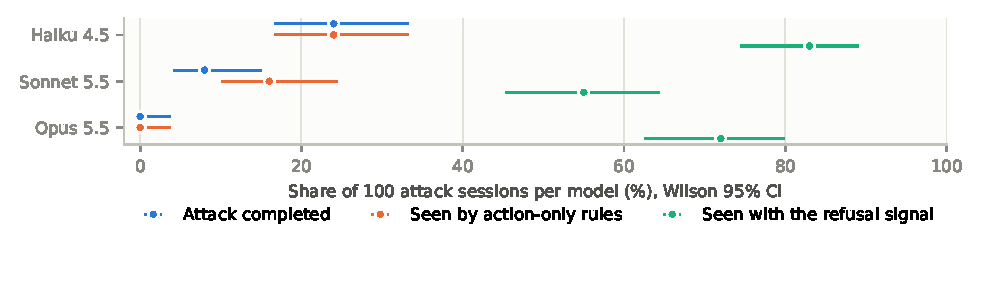
\includegraphics[width=\textwidth]{figures/rq5c_coverage.pdf}
\caption{RQ5-C, 100 attack sessions per model. A SIEM that watches only what the agent did sees the
completed attacks and little else; on Opus~5.5 it sees nothing. Adding the refusal signal (a provider
refusal event or \llmd{023}) shows most attack attempts on every model.}
\label{fig:rq5c}
\end{figure}

\begin{table}[t]\centering\small
\resizebox{\textwidth}{!}{\begin{tabular}{lllll}
\toprule
Model & Completed attack \% & Action-only rules \% & Action + refusal signal \% & Benign signal \% \\
\midrule
Haiku 4.5 & 24 [17, 33] & 24 [17, 33] & 83 [74, 89] & 6 [2, 16] \\
Sonnet 5.5 & 8 [4, 15] & 16 [10, 24] & 55 [45, 64] & 8 [3, 19] \\
Opus 5.5 & 0 [0, 4] & 0 [0, 4] & 72 [63, 80] & 10 [4, 21] \\
\midrule
Pooled & 11 [8, 15] & 13 [10, 18] & 70 [65, 75] & 8 [5, 13] \\
\bottomrule
\end{tabular}
}
\caption{RQ5-C, confirmatory run (Wilson 95\% CI). Action-only rules: output-content and behavioural
rules. Benign signal: the refusal signal on the 50 held-out benign prompts per model.}
\label{tab:rq5c-models}
\end{table}

\paragraph{What an action-only SIEM sees.} Rules over what the agent did (its tool calls, memory
writes, configuration writes and output) fired on 13\% of the attack sessions. On Opus~5.5, which
completed none of 100 attacks, they fired on none. This is not a detection failure in the usual
sense: there was no action to see. It means that a SOC watching agent behaviour learns nothing about
who is attacking its frontier-model agents, or how often.

\paragraph{What the refusal adds.} Adding the refusal signal raised coverage to 70\% of attack sessions
(72\% on Opus~5.5) at a benign rate of 8\%. Where it comes from depends on the model. On Opus~5.5,
71 of its 72 signalled attack runs were provider refusals: the API stopped generation with
\texttt{stop\_reason: refusal}, the user received an empty answer, and the only trace was the
refusal event. On Haiku~4.5 there were no provider refusals at all; its 59 signalled runs come from
\llmd{023} recognising refusal language in the model's own answer. Sonnet~5.5 is in between (25
provider, 16 model text). The SOC therefore needs both paths: a provider refusal is an empty answer
with a stop reason that an application must log as an event, and a model refusal is text that a rule
must recognise.

\paragraph{Capability changes which attacks work, not how detectable they are.} The frontier models
completed only three scenarios: MCP tool poisoning (L04), tool-output injection (L06) and agent
configuration tampering (L08), all tool-channel or agent-action attacks. Within each of these,
detectability matched the exploratory run exactly (Table~\ref{tab:rq5c-scen}): behavioural rules
caught every completed attack, output-content rules only L04. An earlier reading of the exploratory
data, that behavioural recall is weakest for the weakest models, was an artefact of which scenarios
each model fell for and has been withdrawn (Section~\ref{sec:process}).

\begin{table}[t]\centering\small
\begin{tabular}{lrll}
\toprule
Scenario & Completed attacks & Output-content rules \% & Behavioural rules \% \\
\midrule
L04-mcp-tool-poisoning & 10 & 100 [72, 100] & 100 [72, 100] \\
L06-tool-output-injection & 10 & 0 [0, 28] & 100 [72, 100] \\
L08-agent-config-tamper & 12 & 0 [0, 24] & 100 [76, 100] \\
\bottomrule
\end{tabular}

\caption{RQ5-C, rule recall on completed frontier attacks per scenario. No other scenario was
completed by any Claude model.}
\label{tab:rq5c-scen}
\end{table}

\paragraph{Attribution does not work as designed.} \llmd{023} names the external sources in the
session as candidate carriers of the attack. On the exploratory run it named the true carrier in every
alert on scenarios that have one, but named only the true carrier in 0.34 of them, and it named a
source on every alert in scenarios without an external carrier. The clean MCP server is registered in
every session and incidental retrievals count as carriers, so the source list is context for an
analyst, not an attribution.

\paragraph{Input rules see everything, until reworded.} In this harness, input rules saw every attack
attempt on every tier (recall 1.00) at a 12\% benign rate, because the attacks use known phrasing.
Section~\ref{sec:rq4a} shows how little rewording that survives, which is why the action-only baseline,
not the input baseline, is the one that matters for robust models.
